% !TEX encoding = UTF-8
% !TEX TS-program = pdflatex
% !TEX root = ../tesi.tex

%**************************************************************
\section{Sprint 8}
\label{sec:sprint8}
%**************************************************************

%**************************************************************
\subsection{User stories assegnate}
\paragraph{Visualizzazione grafico (8)} \mbox{} \\[\baselineskip]
Come utente autenticato che si trova nella sezione “Reports”, voglio poter vedere un istogramma che rappresenti graficamente i dati contenuti nella tabella.\\

\noindent Tasks:
\begin{itemize}
  \item effettuare una ricerca su quale libreria Javascript possa essere più consona per creare il grafico richiesto;
  \item implementare il grafico.
\end{itemize}

\subsection{Visualizzazione grafico}
Per quanto riguarda la ricerca ho fatto un foglio Google simile a quello già fatto per i datepicker in cui ho raggruppato le librerie che mi sembravano migliori per svolgere l'incarico assegnato:

\begin{itemize}
  \item Chart.js\footcite{site:chartjs}
  \item D3.js\footcite{site:d3}
  \item nivo\footcite{site:nivo}
\end{itemize}

\noindent Chart.js è, tra queste, la libreria più utilizzata e spicca per la sua semplicità di utilizzo e le molteplici tipologie di grafici preconfigurate. Anche il fatto che sia popolare è un punto a favore in quanto dispone di una community più ampia, che porta a trovare con più facilità soluzioni a eventuali problemi riscontrati.\\
Anche D3.js è una libreria piuttosto popolare e non è esclusivamente dedicata alla realizzazione di grafici ma, più in generale, alla manipolazione di elementi del DOM. È caratterizzata da avere un numero altissimo di funzionalità, che si traduce nella capacità di creare grafici complessi e per obiettivi specifici, al prezzo di avere una curva di apprendimento piuttosto ripida.\\
Nivo è basato su D3.js ma offre una buona riduzione di complessità rispetto a quest'ultimo, essendo pensato esclusivamente per la creazione di grafici.\\

La scelta finale è ricaduta su Chart.js in quanto il grafico da produrre era molto semplice e, essendo l'ultima settimana, non ci sarebbe stato tempo per familiarizzare con uno strumento complesso come D3.js.

L'implementazione del grafico si è rivelata infatti piuttosto semplice, dovendo solo dichiarare delle variabili per i dati da mostrare e per delle opzioni aggiuntive del grafico:

\begin{code}[frame=tb, label={code:chart}, caption={Esempio di utilizzo di Chart.js}]\\
1   /*Opzioni aggiuntive del grafico*/
2   const options = {
3     responsive: true,
4     scales: {
5       y: {
6         min: 0,
7       }
8     }
9   };
10
11  /*Dichiarazione dati e relative labels*/
12  const data = {
13    labels: getLabels(),
14    datasets: [
15      {
16        data: getData(),
17      }
18    ]
19  };
20
21  return <Bar options={options} data={data} />;
\end{code}\\\\

\noindent Anche la struttura di come venivano restituiti i dati non è risultata problematica nè per i visualizzare i dati raggruppati nè per quelli non raggruppati.

\subsection{Sprint review}
Essendo la sprint review finale ho dimostrato brevemente le funzionalità sviluppate fino ad ora, ottenendo, anche per quanto riguarda il miglioramento estetico al file PDF assegnatomi lo scorso sprint, un feedback positivo.\\
Nella figura \ref{fig:report_chart} viene mostrato il grafico creato durante lo sprint.
\begin{figure}[H]
	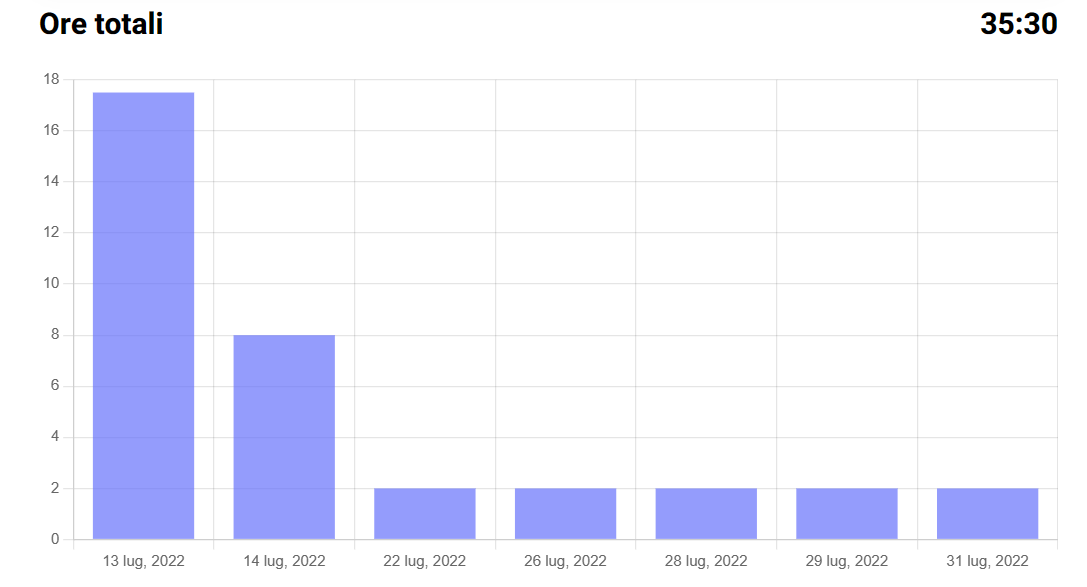
\includegraphics[width = \textwidth]{immagini/reports chart.png}
	\caption{Grafico della sezione Reports}
	\label{fig:report_chart}
\end{figure}